\section{Dataset and Data Analysis}
\label{sec:data}

\subsection{Source and description}
\textbf{HAM10000} (``Human Against Machine with 10{,}000 training images'')~\cite{ham10000} is a multi-source
collection of dermatoscopic images of common pigmented skin lesions. It was gathered over 20 years at the
Medical University of Vienna and at a skin-cancer practice in Queensland, Australia, and it formed the training
set of the ISIC~2018 challenge~\cite{isic2018}. More than half of the diagnoses are confirmed by histopathology;
the rest come from follow-up, expert consensus or in-vivo confocal microscopy. \textbf{DermaMNIST}~\cite{medmnistv2}
repackages the 10{,}015 images as a seven-class benchmark with a fixed 7\,:\,1\,:\,2 train/validation/test split.
We use the \textbf{MedMNIST+ 224$\times$224} release~\cite{medmnistplus}, in which the original
600$\times$450 images are resized to 224$\times$224 RGB (uint8) without cropping.

\begin{table}[H]
\centering
\caption{Dataset facts.}
\label{tab:datafacts}
\small
\begin{tabular}{ll}
\toprule
Source file & \texttt{dermamnist\_224.npz} (Zenodo record 10519652, \DatasetSizeMB\,MB) \\
MD5 (verified) & \texttt{8974907d8e169bef5f5b96bc506ae45d} (matches \texttt{medmnist/info.py}) \\
Images / classes & 10{,}015 RGB images, 7 mutually exclusive diagnostic classes \\
Resolution / type & $224\times224\times3$, uint8 \\
Official split & train 7{,}007 / validation 1{,}003 / test 2{,}005 (stratified, image-level) \\
Licence & CC BY-NC 4.0 (non-commercial research and teaching use) \\
\bottomrule
\end{tabular}
\end{table}

\subsection{Class distribution and imbalance}
Table~\ref{tab:classes} and Figure~\ref{fig:classdist} show a severe long-tailed imbalance. Melanocytic nevi
(\texttt{nv}) make up \textbf{67.0\%} of the training images, while dermatofibroma (\texttt{df}) has only 80
training images (1.1\%). The majority-to-minority ratio is \textbf{58.7\,:\,1}. Three classes are malignant or
pre-malignant (\texttt{akiec}, \texttt{bcc}, \texttt{mel}); together they are only 19.5\% of the data. The split
is stratified, so all three splits share the same class proportions. The validation split has only 12
\texttt{df} and 14 \texttt{vasc} images, which makes per-epoch validation scores for those classes noisy.

\begin{table}[H]
\centering
\caption{Class distribution of DermaMNIST (official splits).}
\label{tab:classes}
\small
\setlength{\tabcolsep}{4pt}
\begin{tabular}{l>{\raggedright\arraybackslash}p{4.6cm}lrrrrr}
\toprule
Code & Diagnosis & Malignant & Train & Val & Test & Total & Share \\
\midrule
\texttt{akiec} & Actinic keratoses / intraepithelial carcinoma & pre-malignant & 228 & 33 & 66 & 327 & 3.3\% \\
\texttt{bcc} & Basal cell carcinoma & yes & 359 & 52 & 103 & 514 & 5.1\% \\
\texttt{bkl} & Benign keratosis-like lesions & no & 769 & 110 & 220 & 1{,}099 & 11.0\% \\
\texttt{df} & Dermatofibroma & no & 80 & 12 & 23 & 115 & 1.1\% \\
\texttt{mel} & Melanoma & yes & 779 & 111 & 223 & 1{,}113 & 11.1\% \\
\texttt{nv} & Melanocytic nevi & no & 4{,}693 & 671 & 1{,}341 & 6{,}705 & 67.0\% \\
\texttt{vasc} & Vascular lesions & no & 99 & 14 & 29 & 142 & 1.4\% \\
\midrule
 & \textbf{Total} & & \textbf{7{,}007} & \textbf{1{,}003} & \textbf{2{,}005} & \textbf{10{,}015} & 100\% \\
\bottomrule
\end{tabular}
\end{table}

\begin{figure}[H]
\centering
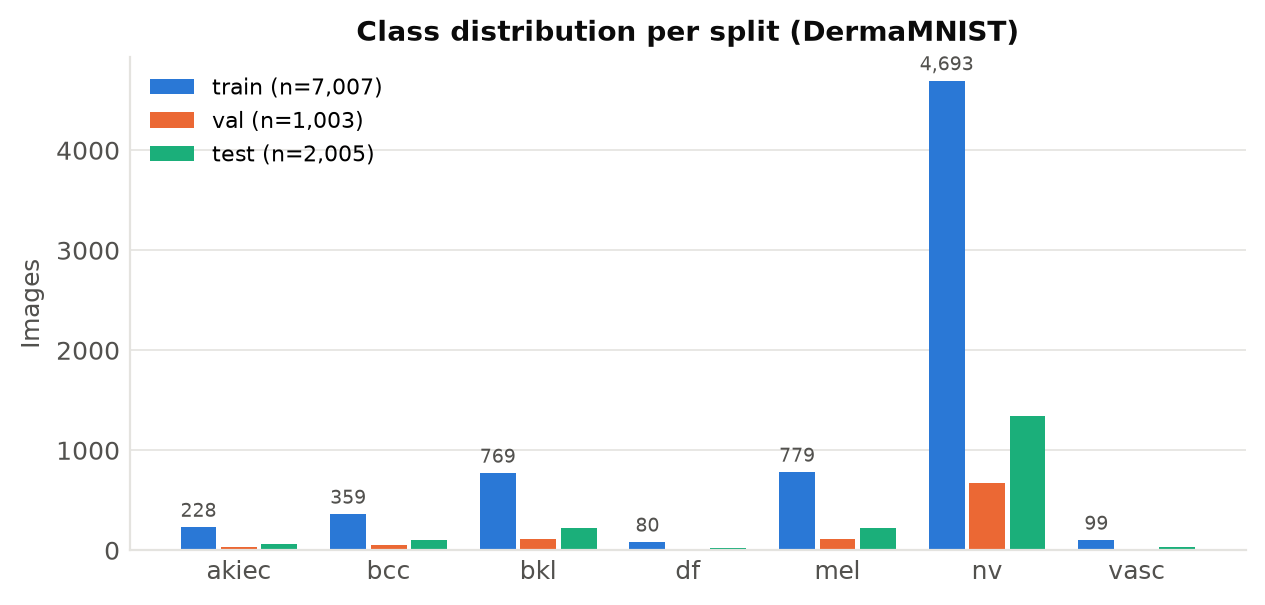
\includegraphics[width=0.82\textwidth]{../results/figures/eda_class_distribution.png}
\caption{Images per class and split. The \texttt{nv} class dominates every split; \texttt{df} and
\texttt{vasc} have fewer than 30 test images each.}
\label{fig:classdist}
\end{figure}

\textbf{Consequences for modelling.} (i)~A classifier that always answers \texttt{nv} already scores
\MajorityAcc\% test accuracy but a macro-F1 of only 0.11, so accuracy cannot be the selection metric; we select
on validation \emph{macro-F1}. (ii)~Rare classes need explicit help, so we use inverse-frequency class weights
in the loss (ablated in Section~\ref{sec:ablation}). (iii)~With 23--29 test images, per-class scores for
\texttt{df} and \texttt{vasc} carry wide uncertainty, so we report bootstrap confidence intervals.

\subsection{Visual inspection}
Figure~\ref{fig:samples} shows random training images. They vary a lot in illumination, zoom and skin tone.
Typical acquisition artefacts are dark circular \emph{vignetting} from the dermatoscope lens, hairs and
occasional reference objects in the field of view (e.g.\ in one \texttt{df} image). The classes overlap visually: many \texttt{mel}, \texttt{nv} and
\texttt{bkl} lesions are brown, roughly round pigmented blobs, and they differ mainly in fine texture, border
irregularity and colour variegation. Vascular lesions (\texttt{vasc}) stand out by their red/purple hue. The
lesion is almost always centred, and orientation is arbitrary. This motivates flip and 90\textdegree-rotation
augmentation, which leaves the label unchanged.

\begin{figure}[H]
\centering
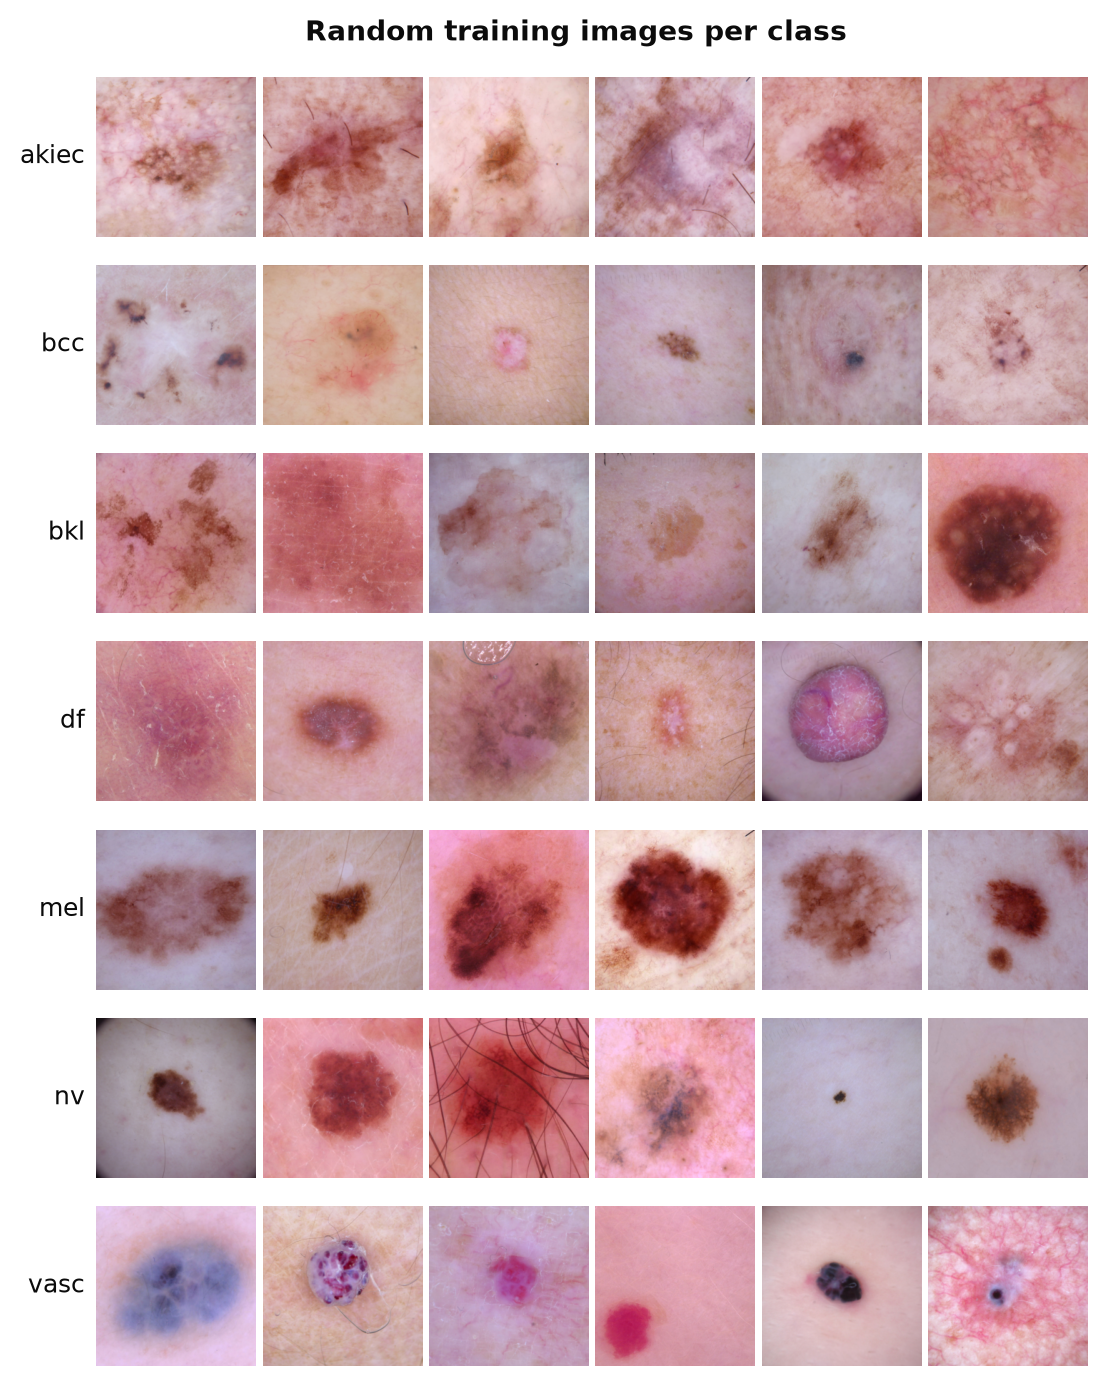
\includegraphics[width=0.70\textwidth]{../results/figures/eda_samples.png}
\caption{Six random training images per class (rows). Note vignetting, hairs and the strong visual similarity
of \texttt{mel}, \texttt{nv} and \texttt{bkl}.}
\label{fig:samples}
\end{figure}

\subsection{Colour statistics}
Over the training split, the per-channel mean (R, G, B) is (0.763, 0.538, 0.562) and the standard deviation is
(0.137, 0.159, 0.177). The images are red-dominant skin tones, quite unlike the ImageNet statistics
(0.485, 0.456, 0.406), which is one aspect of the \emph{domain shift} that fine-tuning has to bridge. We still
normalise with the ImageNet statistics, because the pretrained filters expect inputs on that scale.
Figure~\ref{fig:colour} shows that colour carries class information. Melanoma and benign keratoses are the
darkest classes (median luminance 0.584 and 0.592), while basal cell carcinoma is the brightest (0.668);
\texttt{vasc} and \texttt{bcc} have the highest blue component. The per-class mean images
(Figure~\ref{fig:meanimg}) confirm that lesions are centred. The pigmented classes (\texttt{mel},
\texttt{nv}, \texttt{bkl}) have a dark brown centre, and the \texttt{mel} blob is the darkest and widest.
\texttt{akiec}, \texttt{bcc} and \texttt{df} are only faintly pink, being less pigmented, and \texttt{vasc}
has a distinctly purple centre. Because colour is informative but also depends on the acquisition device, we use only \emph{mild}
colour jitter (Section~\ref{sec:workflow}). Strong jitter could erase real diagnostic cues.

\begin{figure}[H]
\centering
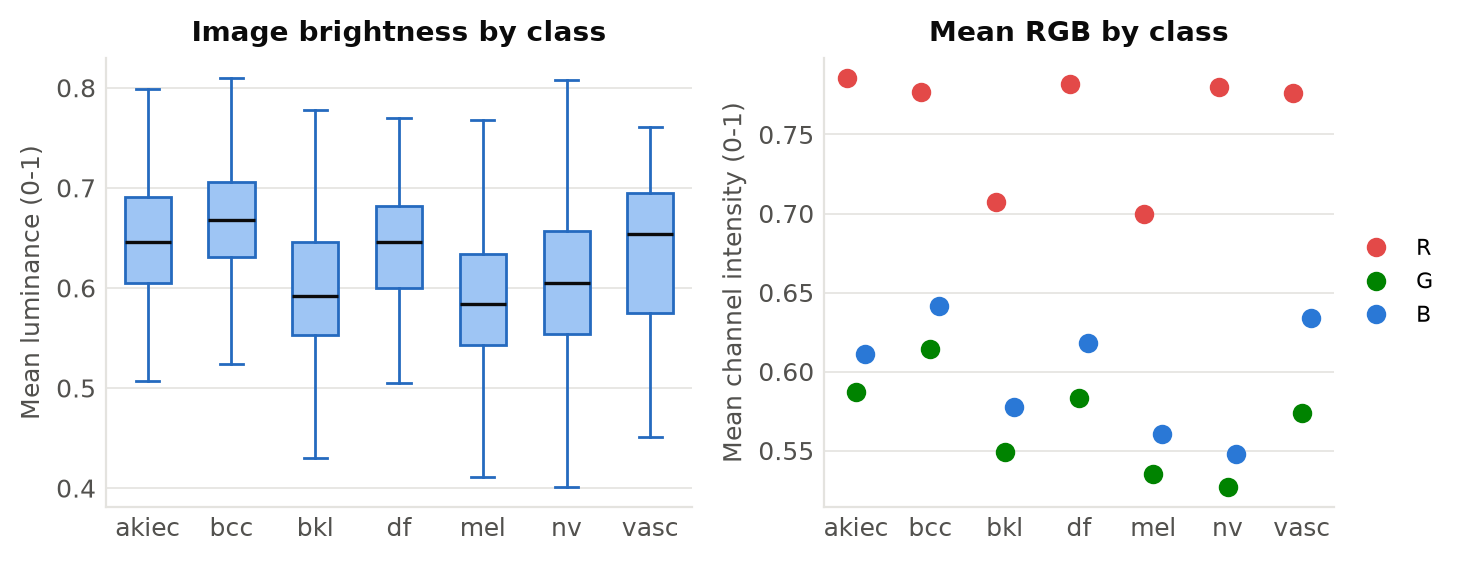
\includegraphics[width=0.92\textwidth]{../results/figures/eda_colour_stats.png}
\caption{Left: distribution of per-image mean luminance by class (boxes = IQR, whiskers = 1.5\,IQR).
Right: mean R, G, B intensity by class.}
\label{fig:colour}
\end{figure}

\begin{figure}[H]
\centering
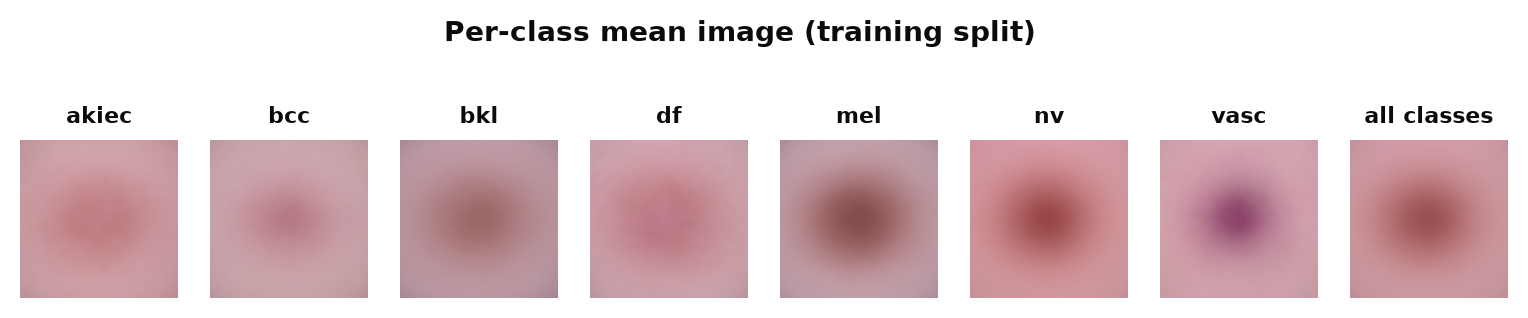
\includegraphics[width=0.98\textwidth]{../results/figures/eda_mean_images.png}
\caption{Pixel-wise mean image per class (training split). Lesions are centred; pigmented classes have a
brown centre (darkest and widest for \texttt{mel}), and \texttt{vasc} a purple one.}
\label{fig:meanimg}
\end{figure}

\subsection{Split integrity: duplicate and leakage audit}
\label{sec:leakage}
HAM10000 often contains \emph{several images of the same lesion}~\cite{ham10000}, and the DermaMNIST split is made
per image, not per lesion. Lesion identifiers are not distributed with DermaMNIST, so we audited the splits
directly in two ways:
\begin{enumerate}
  \item \textbf{Exact duplicates} (MD5 of raw pixels): \textbf{none} of the validation or test images is a
        byte-identical copy of a training image.
  \item \textbf{Near duplicates}: a 64-bit difference hash (dHash) of each image, then the Hamming distance to
        the nearest training image (Table~\ref{tab:dhash}).
\end{enumerate}

\begin{table}[H]
\centering
\caption{Near-duplicate audit with a 64-bit dHash. ``Label agreement'' is the share of pairs whose nearest
training image has the same diagnosis; the last row is the base rate over all images.}
\label{tab:dhash}
\small
\begin{tabular}{lrrrr}
\toprule
 & \multicolumn{2}{c}{Validation (n = 1{,}003)} & \multicolumn{2}{c}{Test (n = 2{,}005)} \\
\cmidrule(lr){2-3}\cmidrule(lr){4-5}
Distance to nearest train image & pairs & label agreement & pairs & label agreement \\
\midrule
$d = 0$ & 3 & 100\% & 3 & 100\% \\
$d \le 2$ & 15 & 73.3\% & 29 & 69.0\% \\
$d \le 4$ & 63 & 60.3\% & 122 & 70.5\% \\
any $d$ (base rate) & 1{,}003 & 56.0\% & 2{,}005 & 59.2\% \\
\bottomrule
\end{tabular}
\end{table}

The pairs at $d=0$ always share the label. Figure~\ref{fig:neardup} confirms that several of the closest pairs
are the same lesion photographed twice, with a slightly different shift or zoom. For $d \le 4$, though, label
agreement (60--71\%) is barely above the base rate (56--59\%). Coarse dHash therefore mostly finds
\emph{look-alike} lesions (round brown blobs on pink skin), not re-photographs. Our conclusion: a \emph{small}
amount of same-lesion leakage does exist between the official splits, so test scores may be slightly optimistic.
It cannot be measured exactly without lesion IDs. We keep the official split so that our numbers stay comparable
with published DermaMNIST results, and we list this as a limitation (Section~\ref{sec:limitations}).

\begin{figure}[H]
\centering
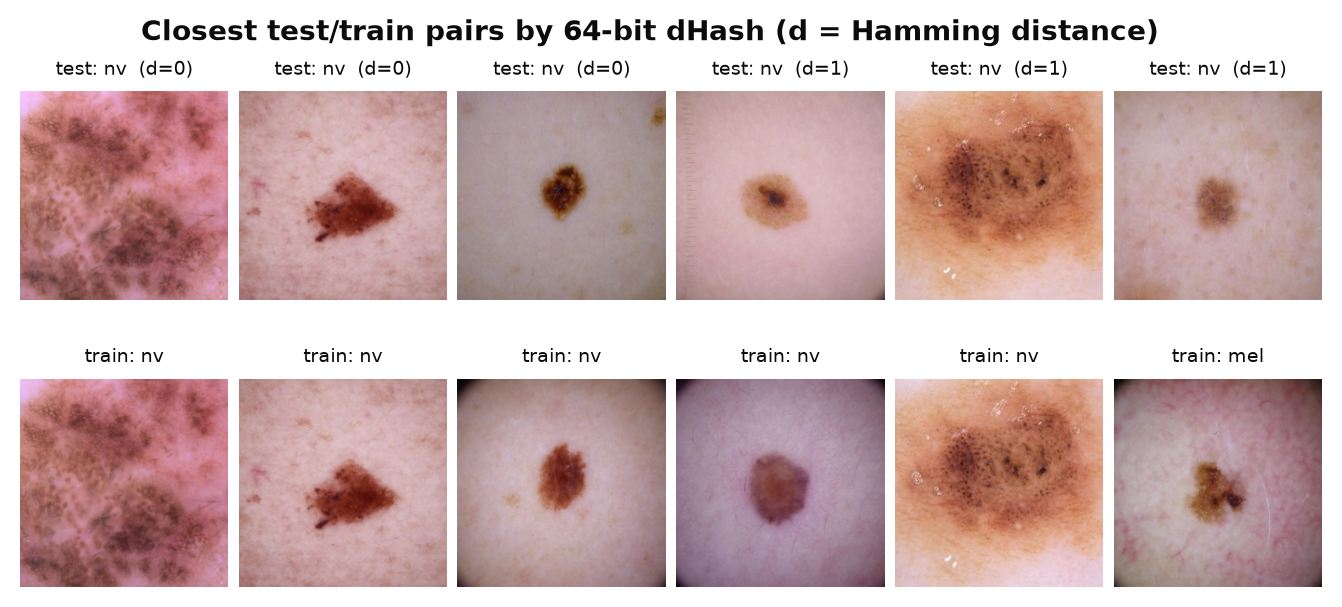
\includegraphics[width=0.85\textwidth]{../results/figures/eda_near_duplicates.png}
\caption{The six test images with the closest training image by dHash (top: test, bottom: nearest train image).
Pairs 1, 2 and 5 are the same lesion re-photographed; pairs 3, 4 and 6 are different lesions.}
\label{fig:neardup}
\end{figure}

\subsection{Summary of data-analysis findings}
\begin{itemize}
  \item Severe imbalance (58.7\,:\,1). We use macro-F1 for model selection and class-weighted loss for training.
  \item Arbitrary lesion orientation. We augment with flips and 90\textdegree{} rotations; the test-time version
        of this becomes 8-view TTA.
  \item Colour is informative but depends on the device. We use only mild colour jitter.
  \item Strong domain shift from ImageNet (colour statistics, texture-dominated content). Full fine-tuning
        should beat frozen features (tested in Section~\ref{sec:performance}).
  \item Small, partly measurable same-lesion leakage in the official splits. We keep it in mind when
        interpreting results.
\end{itemize}
